\chapter{PETUNJUK LAPORAN DARING}
\section{Petunjuk Git Standar}
Diwajibkan pertama kali sebelum anda mengkode adalah membuat terlebih dahulu akun di github, setelah itu buat repositori dari aplikasi yang akan anda bangun,wajib di isi dengan license open source yang ingin anda gunakan dan README.md yang berisi penjelasan aplikasi tersebut, fungsinya, dan penjelasan cara instalasi serta rujukan library yang anda pakai
di aplikasi anda(README.md \textbf{wajib} menggunakan \textbf{bahasa inggris}). Gunakan format markdown untuk membuat README.md anda bisa menggunakan markdown editor online untuk mempermudah pembuatan.
\\
\\
Untuk pengguna windows anda diwajibkan melakukan instalasi git-scm yang diunduh dari situsnya.\\
\url{https://git-scm.com/download/win}\\
\\
\\
Setelah selesai, silahkan melakukan konfigurasi SSH key terlebih dahulu,
untuk melakukan konfigurasi silahkan ikuti langkah-langkah berikut :
\begin{enumerate}
\item Buka terminal git.
\item Ketik "\textit{ssh-keygen}".
\item kita akan diminta mengisi id dan passpharse. Silahkan isi id sesuai dengan keinginan kalian, dan passpharse dapat dikosongkan.
\item Setelah selesai, masuk ke direktori tempat anda menyimpan file tersebut dan buka file yang memiliki ekstensi ".pub" dengan Notepad.
\item Copy semua data yang ada di file tersebut.
\item Lalu buka menu SSH and GPG keys pada Github, dan ssh key yang sudah di copy sebelumnya di kolom key.
\item Lalu klik add SSH key.
\end{enumerate}
Setelah selesai baru anda, bisa memakai repositori dari github yang sudah anda buat di paragraph sebelumnya.\\
Cara penggunaannya :
\begin{enumerate}
\item Buatlah direktori kerja anda untuk mengkode, setelah itu klik kanan 				\textit{"git bash here"} akan mencul terminal git.
\item Ketik "\textit{git init}" untuk menginisiasi repo baru.
\item ambil url remote dari repository yang dibuat. Login terlebih dahulu 		ke github, url remote didapatkan di halaman repositori kita bagian 			\textbf{\underline{clone or download}} pilih \textbf{clone with ssh} 		lalu salin yang ada di textbox. contoh url: 								\url{git@github.com:awangga/nopanel.git}.

\item masukkan remote repository ke direktori kerja kita dengan perintah : 	  \textit{git remote addorigin \url{git@github.com:awangga/						nopanel.git}} .

\item download terlebih dahulu yang sudah ada di repo(license file dan 				readme) dengan perintah: \textit{git pull origin master}.

\item silahkan mulai mengkode, setiap ada perubahan kode yang kita 					inginkan misal menambahkan textbox, maka yang pertama add dahulu 			kemudian commit. contoh : \textit{git add filenya.php} dan 					kemudian \textit{git commit -m "menambahkan textbox"} . Komentar 			harus berarti mengacu pada kode yang diubah bukan asal isi atau 			nilai SCM anda nol.

\item Lakukan berulang langkah 6 untuk setiap perubahan per file 					apapun(dilarang menggunakan \textit{git add . }).

\item Setelah selesai mengkoding anda mengunggahnya ke repo github dengan 			perintah : \textit{git push origin master}.

\item Lakukan berulang langkah 5-8 setiap anda melakukan pengkodean. 				Performansi anda akan terlihat di profile github anda disitu 				pembimbing akan melakukan penilaian secara proses pengkodean 				apakah sesuai dengan metode pengembangan perangkat lunak yang ada 			di proposal atau tidak.

\item Apabila laptop anda hilang. maka anda tinggal mengulangi langkah 1-5 		dan pekerjaan anda tidak ada yang hilang dan masih bisa 					diteruskan.

\item Anda bisa menggunakan branch yang berbeda(dalam repo yang sama) jika
		mengembangkan versi yang berbeda atau ada keraguan dalam 					pengembangan. Selengkapnya tentang branch bisa dibaca disini 				\url{http://www.vas.web.id/2016/08/gitautodelpoy-ke-server-					produksi.html}.
		
\item Jika sudah program sudah matang, maka di rilis dari menu github 				repository.
\end{enumerate}
Untuk	bimbingan	metode	kan-ban	silahkan	buat	project	di	tab	project	seperti	gambar.


\begin{figure}[H]
    \centering
    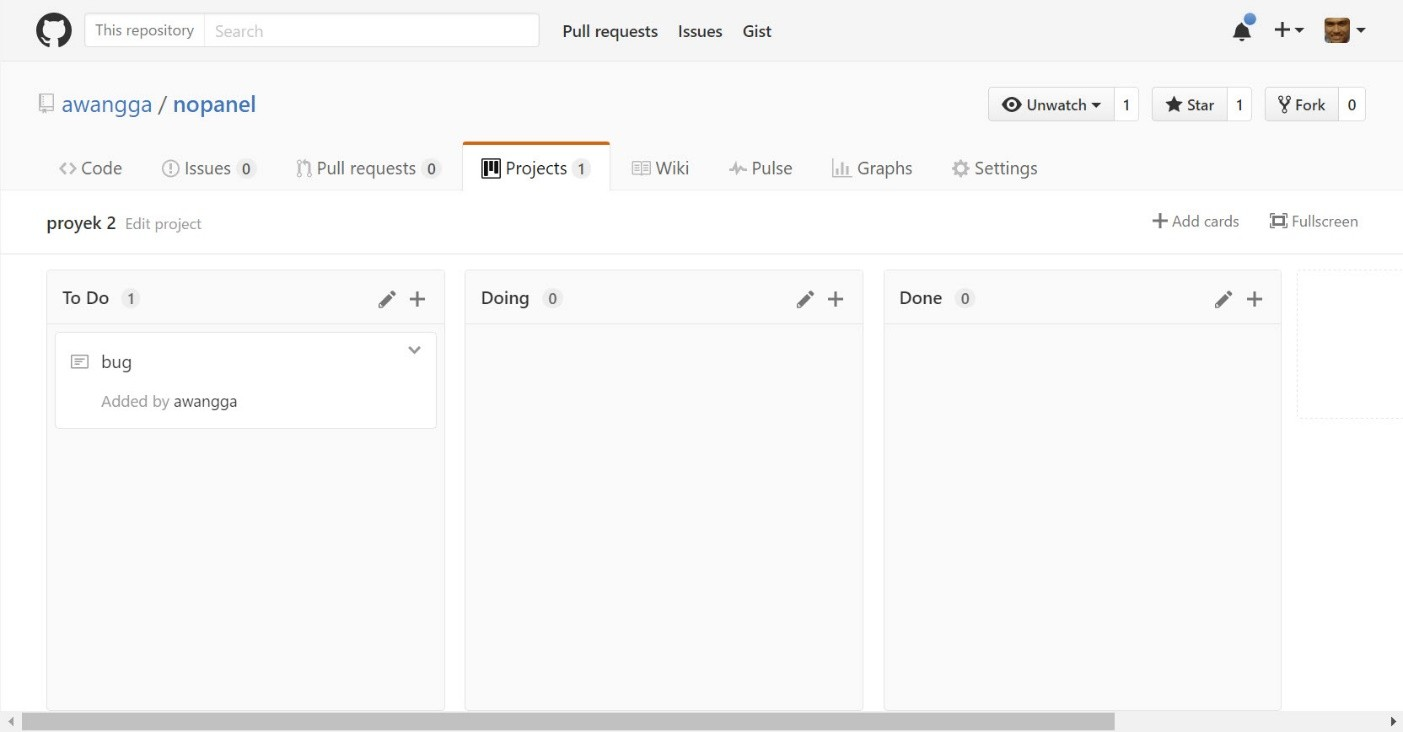
\includegraphics[scale=0.4]{figures/aad.jpg}
    \label{aasd}
\end{figure}

\textbf{\underline{Penting :}}\par
Git	ini	merupakan	alat	kontrol	pengembangan	aplikasi,	ingat!!!	dipakai	sejak	awal	mulai	mengkode	bukan	mengunggahnya	pada	saat	terakhir	sebelum	sidang	atau	anda	mendapat	nilai	0	
untuk	SCM(Source	Code	Management)/	Manajemen	Kode	Sumber.
\par 

Apabila	aplikasi	anda	tidak	dibuka	publik	atau	opensource	bisa	diganti	dengan	bitbucket	atau	
git.vas.web.id
\par 

Petunjuk	standar	github	dalam	bentuk	video	bisa	dibuka	melalui	link	berikut	:
\begin{enumerate}
\item Membuat	repositori	di	github	: \url{https://youtu.be/27JkHR59mmg}
\item Invite	User	: \url{https://youtu.be/gbxW8bQ29y0}
\item Menggunakan	git	scm	: \url{https://youtu.be/DpgfmeCZsCQ}
\end{enumerate}

\section{Petunjuk	Video	Standar}
Video	yang	dibuat	dibagi	menjadi	tiga	bagian	waktu	(linimasa)	dalam	satu	video, \textbf{waktu pembuka} yaitu	mulai	dari	menit	ke	nol,\textbf{waktu	penjelasan} disambung	setelah	waktu	pembuka,\textbf{waktu	penutup} disambung	setelah	waktu	penjelasan.
\\
\\
\textbf{Waktu Pembuka :}
\\
\begin{enumerate}
\item Video	muka	diri	sendiri	ukuran	setengah	badan	atau	lebih,	memperkenalkan	diri	dengan	nama,	kelas,	jurusan	dan	npm	beserta	nama	pembimbing	dan	jelaskan	keunggulan,	kelebihan	dan	kemampuan	anda (\textit{Nilai	20}).

\item . memberikan	latar	belakang	permasalahan	yang	akan	disolusikan	dengan	menggunakan	minimal	satu	alat	peraga	(minimal	papan	tulis	atau	alat	peraga	lainnya	yang	membantu	
penjelasan) (\textit{Nilai	20})
\end{enumerate}

\textbf{Waktu	Penjelasan	:}\\
video	penjelasan	wajib	terdiri	dari \textbf{teori	dan	praktek}.
\begin{enumerate}
\item Penjelasan	teori	menggunakan	alat	peraga, (\textit{Nilai	20})
\item kemudian	praktek	bisa	merekam	layar	laptop	untuk	praktek	pengkodean	atau	merekam	praktek	langsung	kondisi	di	lapangan. (\textit{Nilai	20})
\end{enumerate}

\textbf{Waktu	Penutup	:}
\begin{enumerate}
\item Berisi	kesimpulan	dan	saran (\textit{nilai 20})
\end{enumerate}

\section{Petunjuk	Standar	Tulisan	Blog}
Anda	bisa	menggunakan	blog	yang	digunakan	bersama	dalam	satu	kelompok	atau	kelas	jika	disepakati	seluruh	tulisan	dimasukkan	ke	satu	alamat	blog	saja	oleh	dosen,	atau	jika	diminta	di	blog	masing-masing	anda	bisa	menggunakan	Wordpress.com,	medium.com,kompasiana.com,	blogger.com. \\
Untuk	kepentingan	tugas	dan	bimbingan	dalam	bentuk	tulisan	di	blog,	memiliki	standar	baku	untuk	kerangka	penulisannya	harus	berisi	:\\
\textbf{Pembuka :}
\begin{enumerate}
\item Gambar	Ilustrasi	Buatan	Sendiri	Orisinil	(Nilai	20).
\item Latar	Belakang	Masalah	(nilai	20).
\end{enumerate}

\textbf{Isi :}
\begin{enumerate}
\item Tambahkan \underline{Video Standar} disini(Penilaian	Video	Terpisah).
\item Penjelasan	dan	solusi	masalah	(nilai	20).
\end{enumerate}

\textbf{Penutup :}
\begin{enumerate}
\item Kesimpulan	dan	saran	(nilai	20).

\item Tambahkan	URL \underline{Git	yang	sudah	Standar} disini(Penilaian	Git Terpisah).

\item Tambahkan	Nama,	NPM,	Kelas,	Prodi,	Kampus.

\item Link/URL	dengan	Nama	Matakuliah	diarahkan	ke	http://www.awangga.net/	atau	yg	disepakati	(Contoh	: \underline{Sistem	Informasi	Geografis}).

\item Referensi	atau	daftar	pustaka	(nilai	20).

\item Link/URL	menuju	skrinsut	Hasil	Scan \underline{ Plagiarisme}(Pilih	2	diantara	4	di	menu	Plagiarisme) yang	diupload	di	google	drive	(Wajib	ada,	jika	tidak	ada	atau	nilai	0)

\end{enumerate}

Penting	:	Sebelum	tulisan	anda	di	publish	di	blog,	untuk	di	scan	plagiarisme	terlebih	dahulu.	Seteleh	publish	scan	lagi	dengan	URL	blog	Plagiarisme	Checker.	Nilai	\%	plagiarisme	diambil	yang	paling	rendah	persentasenya. \\
Nilai	akhir	tulisan	=	Total	Nilai	Tulisan	(20+20+20+20+20)*Persentasi	(\%)	Uniqeness	hasil	scan	
plagiarisme.

